\usemintedstyle{tango}
\setminted[python]{fontsize=\footnotesize}
In the first part of this thesis we have established a theoretical basis about multigrid methods, formal languages and genetic programming.
In Chapter~\ref{chapter:multigrid-formal-language}, building on this foundation, we have then developed a novel formal language and grammar for the automatic generation of multigrid methods. 
While we have already demonstrated that the capabilities of this approach in alternating each individual step of a multigrid method, we could not yet demonstrate its benefits compared to the use of classical multigrid cycles, such as V-, F- and W-cycles.
We aim to achieve this goal with the implementation of \emph{EvoStencils}, a prototypical Python framework for the grammar-guided optimization of multigrid methods.
Using this framework we will then show how it is possible to evolve methods that are more efficient than all common multigrid cycles in solving a number of PDE-based problems while being structurally different that any other known method of this type.
However, before we discuss EvoStencils' features and their implementation in Python, we want to provide an overview about its workflow and software architecture.
In general, we can distinguish between EvoStencils' core implementation and the functionality of the framework that is build upon the use of external libraries.
First of all, since our formulation of the rules to construct a multigrid methods in the form of a context-free grammar, we can utilize the grammar-guided genetic programming techniques presented Chapter~\ref{chapter:formal-languages-and-gp} without adapting their inner workings.
For this purpose, we employ the widely-used evolutionary computation framework DEAP\footnote{DEAP: \url{https://github.com/deap/deap}}~\cite{rainville2012deap}, which enables us to implement GGGP in a modular way while requiring only a limited amount of adaption.
However, the questions that then remains to be answered how we can evaluate each multigrid method obtained through GGGP in an automatic and reproducible manner.
As we have seen in Section~\ref{sec:grammar-based-algorithm-generation} the 
application of the sequence of state transition functions represented in a given derivation tree produces a computational graph of the form of Figure~\ref{fig:example-three-grid-method-computational-graph}, which can then be transformed to an algorithmic representation, as shown in Algorithm~\ref{alg:example-three-grid-method-generated}.
However, while any expert could now manually implement the corresponding multigrid solver based on this representation using an arbitrary numerical software package, within GGGP we have to evaluate each method in an automatic way without requiring any human intervention.
Recently, code-generation techniques based on the specification of a numerical solver in a high-level domain specific language (DSL) have become increasingly powerful~\cite{kostler2020code}.
An example for this approach is the ExaStencils framework~\cite{lengauer2020exastencils,lengauer2014exastencils}, which has been specifically designed for the automatic generation of fast and scalable implementation of multigrid-based solvers specified in a tailored DSL called ExaSlang~\cite{schmitt2014exaslang,schmitt2016systems,kuckuk2016automatic}.
ExaSlang enables the formulation of a multigrid method as a sequence of high-level operations, without the need to consider the implementation details of each individual statement, while still granting the user the flexibility to apply further optimizations through the addition of code transformations and lower-level statements.
To evaluate a given solver, obtained from a grammar-based representation, we, therefore, emit its corresponding algorithmic formulation as an ExaSlang specification, based on which we then employ the ExaStencils framework to generate a scalable C++ implementation.
The resulting program can then be executed on a number of test cases in order to measure the desired performance characteristics of the solver.
Finally, note that the execution of a GGGP-based optimization approach requires the evaluation of a large number of different multigrid methods.
Depending on the problem that one aims to solve it can be infeasible to perform the optimization on a single compute node, necessitating the implementation of a multi-node parallelization.
The message passing interface (MPI)~\cite{walker1996mpi} provides a unified interface for performing parallel computations on a distributed system that is supported by the majority of supercomputing devices available.
While MPI has been originally designed for the traditional scientific computing languages Fortran and C, it recently has been also made available within Python~\cite{dalcin2021mpi4py}. 
With the addition of MPI, as a distributed computing backend, we arrive at the following high-level view of EvoStencils' software architecture, which is shown in Figure~\ref{fig:evostencils-architecture}.
\begin{figure}
	\resizebox{\columnwidth}{!}{%
		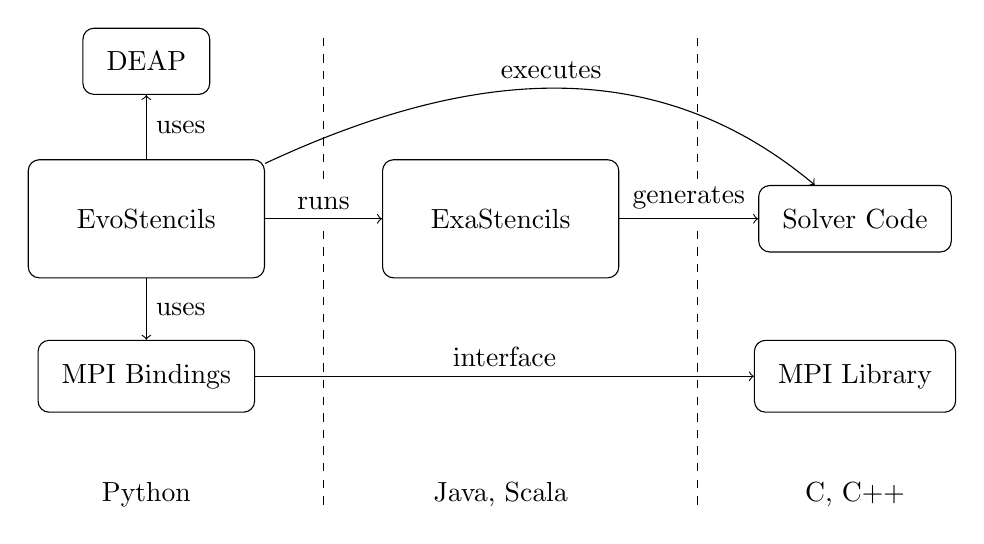
\begin{tikzpicture}
			%\draw [help lines] (-10,-10) grid (10,10);
			\node[draw, minimum width=3cm, minimum height=1.5cm, rounded corners] (evo) at (0,0) {EvoStencils};
			\node[draw, inner sep=3mm, rounded corners] (bindings) at (0, -2) {MPI Bindings};
			\node[draw, inner sep=3mm, rounded corners] (deap) at (0, 2) {DEAP};
			\node[draw, minimum width=3cm, minimum height=1.5cm, rounded corners] (exa) at (4.5, 0) {ExaStencils};
			\node[draw, inner sep=3mm, rounded corners] (code) at (9, 0) {Solver Code};
			\node[draw, inner sep=3mm, rounded corners] (mpi) at (9, -2) {MPI Library};
			\draw[dashed] (2.25, 2.3) -- (2.25,0.5);
			\draw[dashed] (2.25, -0.15) -- (2.25,-3.7);
			\draw[dashed] (7, 2.3) -- (7,0.5);
			\draw[dashed] (7, -0.15) -- (7,-3.7);
			\node (python) at (0, -3.5) {Python};
			\node (java) at (4.5, -3.5) {Java, Scala};
			\node (c) at (9, -3.5) {C, C++};
			\draw[->] (evo)-- node[anchor=west] {uses} (deap);
			\draw[->] (evo)-- node[anchor=south]{runs} (exa);
			\draw[->] (exa)--node[anchor=south] {generates} (code);
			\draw[->] (evo) to [out=25,in=140] node[anchor=south] {executes} (code);
			\draw[->] (bindings)--node[anchor=south] {interface}(mpi);
			\draw[->] (evo)--node[anchor=west] {uses}(bindings);
			%\draw[->] (mpi)--(code);
		\end{tikzpicture}
	}\caption{Software Architecture of EvoStencils.}
	\label{fig:evostencils-architecture}
\end{figure}
In the following, we will now consider the individual parts of this architecture in more detail, starting with the core implementation of EvoStencils, which can be considered as a separate module that does not depend on any of the other tools and libraries mentioned here.
As a first step, we will outline the implementation of an intermediate representation for multigrid methods that can be easily obtained from a given derivation tree and which then acts as a basis for all subsequent steps of solver generation and evaluation.

\section{Intermediate Representation}
\begin{listing}
	\inputminted{python}{evostencils/ir/grid.py}
	\caption{Class for Representing Uniform Grids}
\end{listing}
\begin{listing}
	\inputminted{python}{evostencils/ir/expression.py}
	\caption{Abstract Expression Base Class}
\end{listing}
\begin{listing}
	\inputminted{python}{evostencils/ir/entity.py}
	\caption{Base Class for Representing Entities}
\end{listing}
\begin{listing}
	\inputminted{python}{evostencils/ir/unary_expression.py}
	\caption{Base Class for Representing Unary Expressions}
\end{listing}
\begin{listing}
	\inputminted{python}{evostencils/ir/binary_expression.py}
	\caption{Base Class for Representing Binary Expressions}
\end{listing}